\documentclass[tikz,border=4pt]{standalone}
\usepackage{pifont}
\usetikzlibrary{positioning,calc,arrows.meta}
\definecolor{accB}{HTML}{1769AA}
\definecolor{fillB}{HTML}{DCEAF5}
\definecolor{accO}{HTML}{C85A00}
\definecolor{fillO}{HTML}{FCE8D5}
\definecolor{ink}{HTML}{18212B}
\definecolor{slate}{HTML}{66727D}
\definecolor{chipgray}{HTML}{D9DEE3}
\definecolor{bad}{HTML}{B83232}
\definecolor{good}{HTML}{3A7D44}
% note (luojiaxuan): 放大版 teaser——行标签移到行上方、结果标记移到行下方,
% 横向足迹从 ~11cm 压到 ~7cm,同一 \columnwidth 下主体放大约五成。
\newcommand{\evcard}[3]{% x, y, style: 0=summary,1=recent,2=distant
  \ifnum#3=0
    \draw[slate, dashed, rounded corners=1.5pt, fill=white]
      (#1-0.26,#2-0.34) rectangle (#1+0.26,#2+0.34);
  \fi
  \ifnum#3=1
    \draw[accB, very thick, rounded corners=1.5pt, fill=fillB]
      (#1-0.26,#2-0.34) rectangle (#1+0.26,#2+0.34);
  \fi
  \ifnum#3=2
    \draw[accO, very thick, rounded corners=1.5pt, fill=fillO]
      (#1-0.26,#2-0.34) rectangle (#1+0.26,#2+0.34);
  \fi
  \fill[chipgray] (#1-0.18,#2-0.27) rectangle (#1+0.18,#2-0.13);
}
\begin{document}
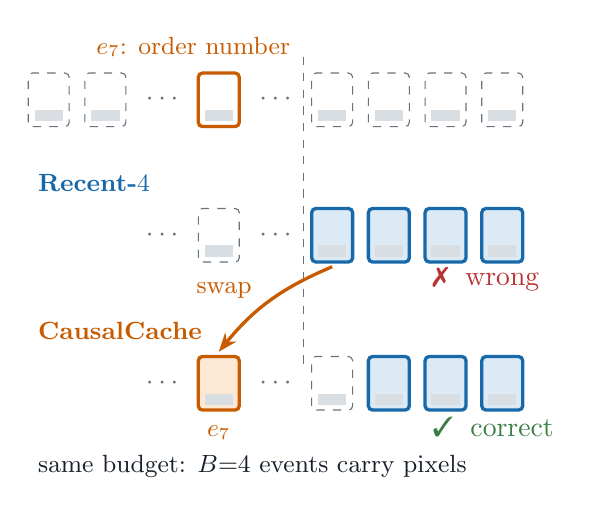
\begin{tikzpicture}[
  font=\normalsize,
  arr/.style={-{Stealth[length=2.4mm]}, ink, semithick},
]
\def\dx{0.72}

%% ---------- episode:e1 e2 ··· e7 ··· 最近4 ----------
\foreach \i in {1,2} {\evcard{\dx*\i}{0}{0}}
\node[font=\normalsize, text=slate] at (\dx*3,0) {$\cdots$};
\evcard{\dx*4}{0}{0}
\node[font=\normalsize, text=slate] at (\dx*5,0) {$\cdots$};
\foreach \i in {6,...,9} {\evcard{\dx*\i}{0}{0}}
\node[font=\small, text=accO, anchor=south] at (\dx*3.55, 0.42)
  {$e_7$: order number};
\draw[accO, very thick, rounded corners=1.5pt]
  (\dx*4-0.26,-0.34) rectangle (\dx*4+0.26,0.34);
% recent window 分界
\draw[slate, dashed] (\dx*5.5, 0.55) -- (\dx*5.5, -3.42);

%% ---------- Recent-4 ----------
\def\rowy{-1.72}
\node[font=\small\bfseries, text=accB, anchor=west] at (\dx*1-0.26, \rowy+0.66)
  {Recent-$4$};
\node[font=\normalsize, text=slate] at (\dx*3,\rowy) {$\cdots$};
\evcard{\dx*4}{\rowy}{0}
\node[font=\normalsize, text=slate] at (\dx*5,\rowy) {$\cdots$};
\foreach \i in {6,...,9} {\evcard{\dx*\i}{\rowy}{1}}
\node[font=\normalsize, text=bad, anchor=west] at (\dx*7.6, \rowy-0.56)
  {\ding{55}\; wrong};

%% ---------- CausalCache ----------
\def\rowyy{-3.6}
\node[font=\small\bfseries, text=accO, anchor=west] at (\dx*1-0.26, \rowyy+0.66)
  {\textsc{CausalCache}};
\node[font=\normalsize, text=slate] at (\dx*3,\rowyy) {$\cdots$};
\evcard{\dx*4}{\rowyy}{2}
\node[font=\normalsize, text=slate] at (\dx*5,\rowyy) {$\cdots$};
\evcard{\dx*6}{\rowyy}{0}
\foreach \i in {7,8,9} {\evcard{\dx*\i}{\rowyy}{1}}
\node[font=\small, text=accO, anchor=north] at (\dx*4, \rowyy-0.42) {$e_7$};
\node[font=\normalsize, text=good, anchor=west] at (\dx*7.6, \rowyy-0.56)
  {\ding{51}\; correct};
% swap 箭头
\draw[arr, accO, very thick] ($(\dx*6, \rowy-0.4)$) to[bend right=14]
  ($(\dx*4, \rowyy+0.4)$);
\node[font=\small, text=accO, anchor=east] at (\dx*4.75, -2.42) {swap};
% 预算标注
\node[font=\small, text=ink, anchor=west] at (\dx*1-0.26, \rowyy-1.06)
  {same budget: $B{=}4$ events carry pixels};
\end{tikzpicture}
\end{document}
